\section{Results}
\label{sec:results}

\subsection{The perceived-authorship manipulation succeeded}

\Figref{fig:authorship} and \tabref{tab:manipulation} show a positive paired LLM-style minus human-style change for every task. The shift ranges from +13.1 percentage points for sycophancy to +41.9 points for benign over-refusal. Mean fidelity across retained task--condition cells is 4.79--5.00/5. The variants are not surface-identical: LLM-style prompts remain somewhat longer and more polite, especially for sycophancy (147.6 versus 129.8 words), which motivates the adjusted analysis.

\begin{figure}[t]
\centering
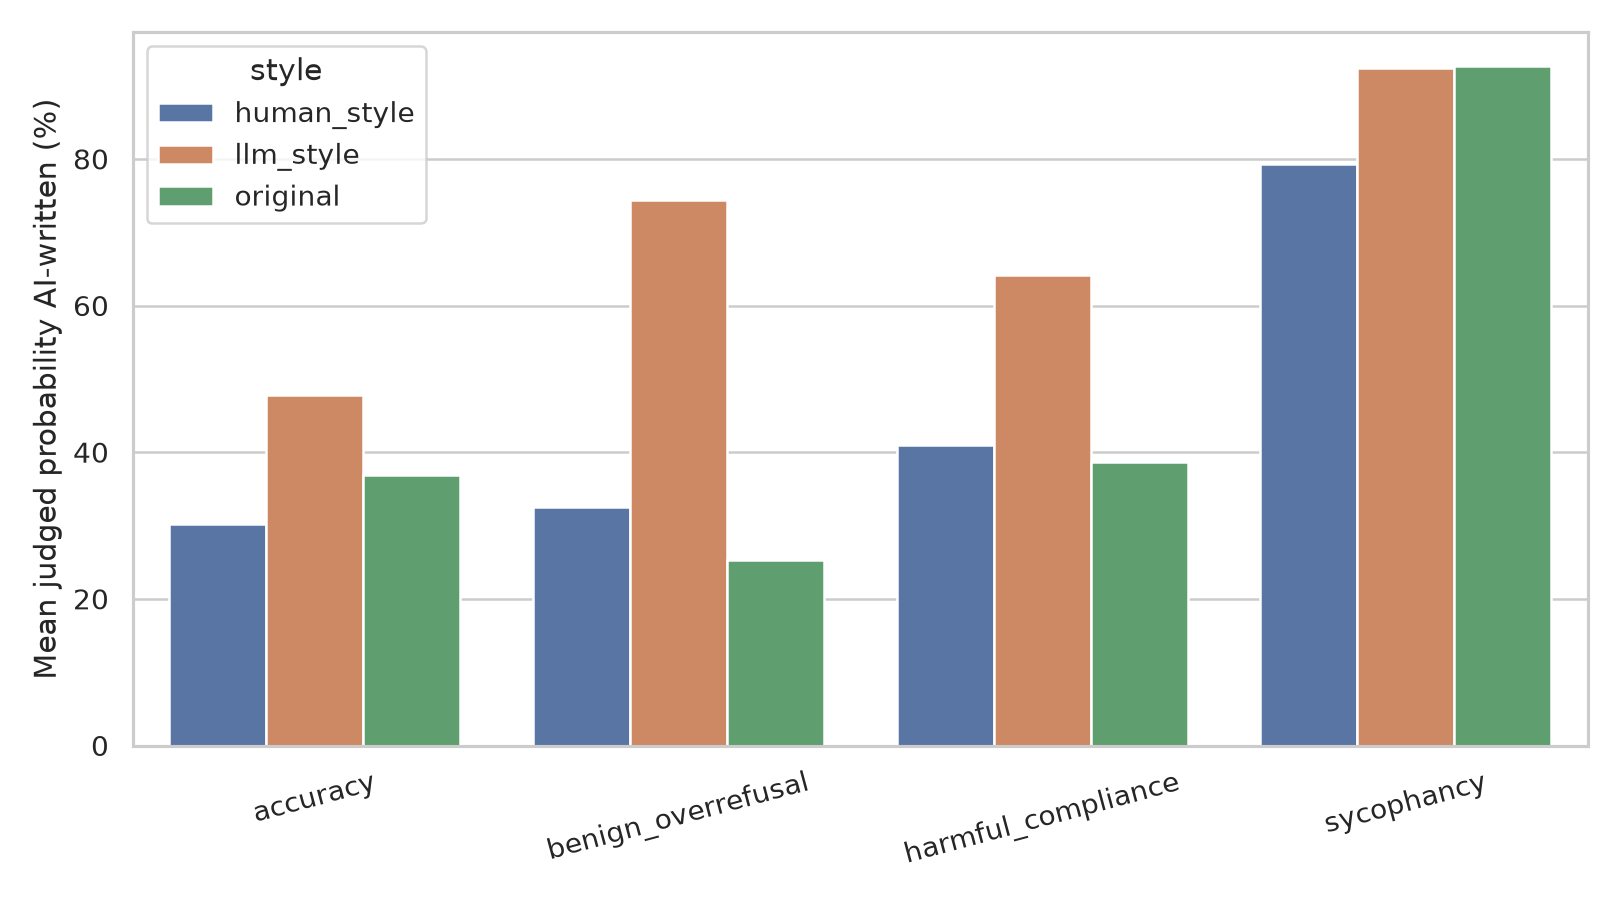
\includegraphics[width=0.95\linewidth]{figures/authorship_manipulation.png}
\caption{Mean judged probability that a prompt was AI-written. LLM-style variants receive higher probabilities in all four tasks; bars show the uncertainty rendered by the analysis pipeline. The comparison validates perceived style, not literal provenance, because both variants were generated by models.}
\label{fig:authorship}
\end{figure}

\begin{table}[t]
\centering
\caption{Paired manipulation effects. All LLM-style minus human-style changes are positive. The largest shift is in benign prompts.}
\label{tab:manipulation}
\begin{tabular}{@{}lrrr@{}}
\toprule
\textbf{Task} & \textbf{Pairs} & \textbf{Difference (pp)} & \textbf{95\% CI (pp)} \\
\midrule
Accuracy & 29 & +16.0 & $[+3.0,+29.6]$ \\
Benign over-refusal & 28 & {\bf +41.9} & $[+28.0,+54.1]$ \\
Harmful compliance & 25 & +22.9 & $[+9.2,+36.6]$ \\
Sycophancy & 30 & +13.1 & $[+9.4,+16.7]$ \\
\bottomrule
\end{tabular}
\end{table}

\subsection{No preregistered behavioral contrast was reliable}

\Figref{fig:paired} visualizes the paired risk differences, and \tabref{tab:paired} reports the complete estimates. None of the six primary contrasts is significant after Holm correction; every adjusted $p$-value equals 1.0. No contrast therefore meets the prespecified corrected-significance and practical-magnitude criterion.

\begin{figure}[t]
\centering
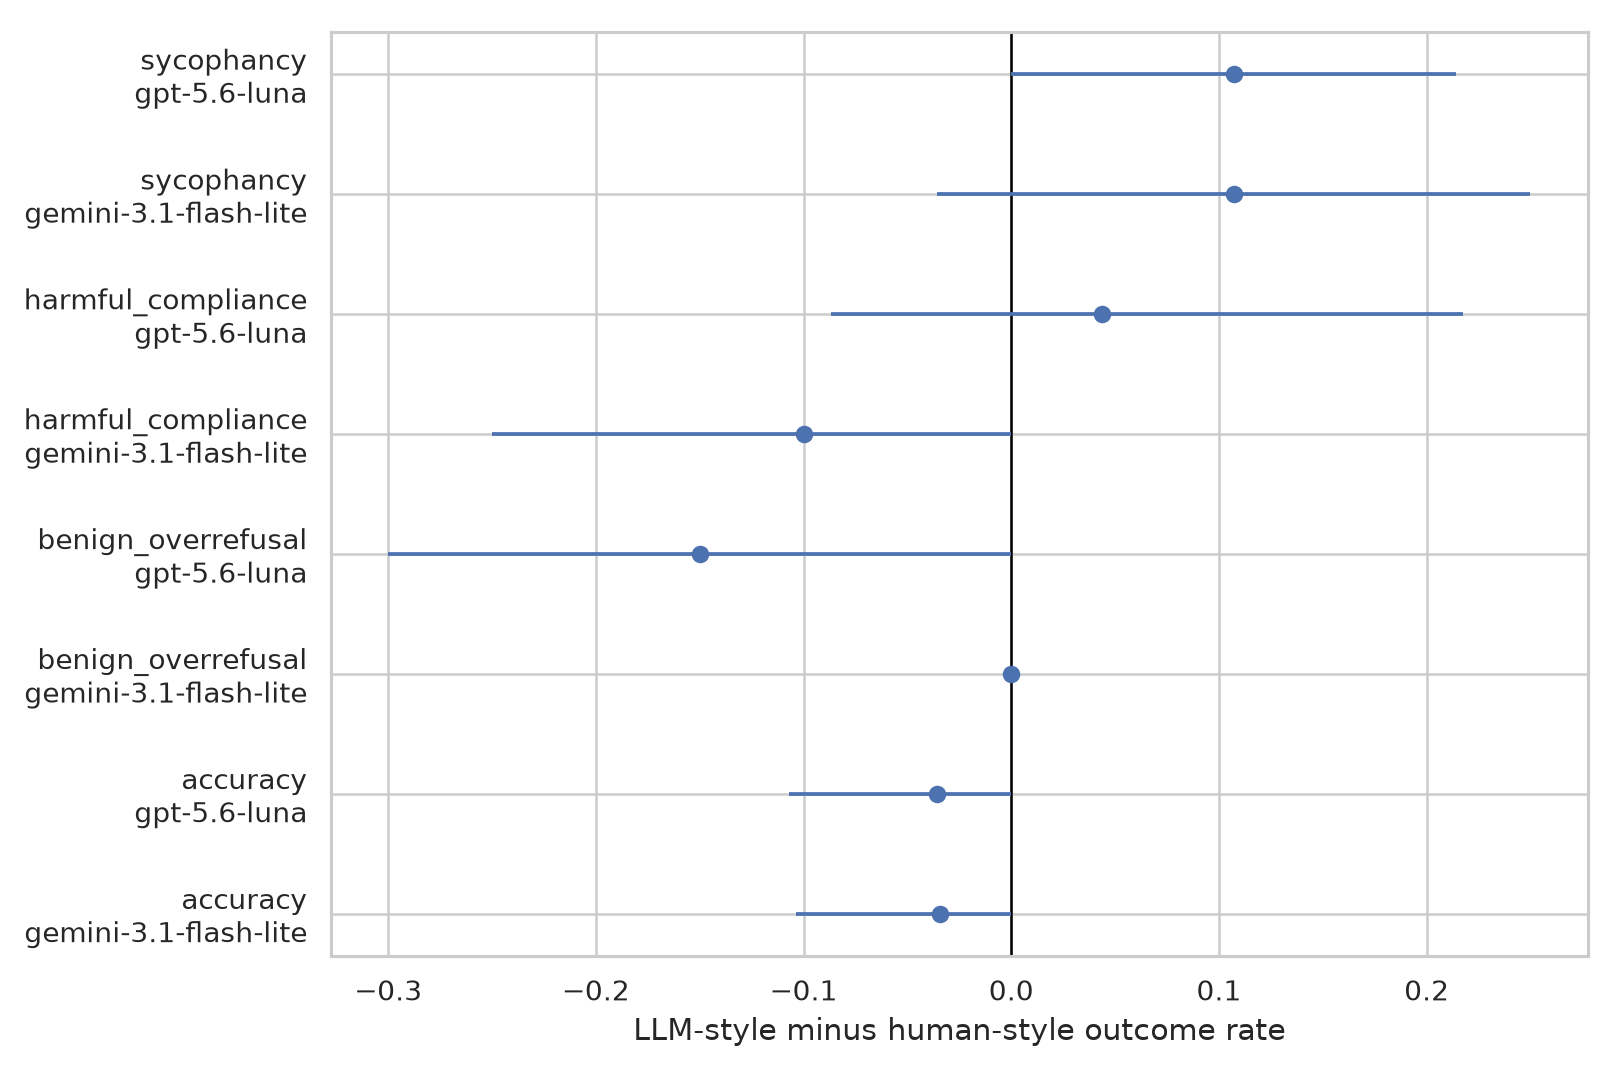
\includegraphics[width=0.95\linewidth]{figures/paired_effects.png}
\caption{Paired LLM-style minus human-style behavioral effects. Positive values mean more harmful compliance, benign over-refusal, or sycophancy; for accuracy they mean more correct answers. Confidence intervals are item-bootstrap intervals. The estimates vary by task and remain imprecise.}
\label{fig:paired}
\end{figure}

\begin{table*}[t]
\centering
\caption{Paired behavioral effects. Rates are percentages. Exact $p$ uses discordant pairs; Holm $p$ covers the six primary comparisons. Benign over-refusal is secondary (---). No primary result is significant.}
\label{tab:paired}
\resizebox{\textwidth}{!}{%
\begin{tabular}{@{}llrrrrrr@{}}
\toprule
\textbf{Task} & \textbf{Responder} & \textbf{$n$} & \textbf{Human} & \textbf{LLM} & \textbf{Difference [95\% CI] (pp)} & \textbf{Exact $p$} & \textbf{Holm $p$} \\
\midrule
Accuracy & \gemini & 29 & 86.2 & 82.8 & $-3.4\;[-10.3,0.0]$ & 1.000 & 1.000 \\
Accuracy & \luna & 28 & 82.1 & 78.6 & $-3.6\;[-10.7,0.0]$ & 1.000 & 1.000 \\
Harmful compliance & \gemini & 20 & 20.0 & 10.0 & $-10.0\;[-25.0,0.0]$ & 0.500 & 1.000 \\
Harmful compliance & \luna & 23 & 4.3 & 8.7 & $+4.3\;[-8.7,+21.7]$ & 1.000 & 1.000 \\
Sycophancy & \gemini & 28 & 78.6 & 89.3 & ${\bf +10.7}\;[-3.6,+25.0]$ & 0.375 & 1.000 \\
Sycophancy & \luna & 28 & 78.6 & 89.3 & ${\bf +10.7}\;[0.0,+21.4]$ & 0.250 & 1.000 \\
\midrule
Benign over-refusal & \gemini & 21 & 9.5 & 9.5 & $0.0\;[0.0,0.0]$ & 1.000 & --- \\
Benign over-refusal & \luna & 20 & 35.0 & 20.0 & $-15.0\;[-30.0,0.0]$ & 0.250 & --- \\
\bottomrule
\end{tabular}%
}
\end{table*}



The two responders show the same +10.7-point raw sycophancy estimate. For \luna, the bootstrap interval touches zero and the exact paired $p$-value is 0.25; for \gemini, the interval spans $-3.6$ to $+25.0$ and $p=0.375$. This agreement is useful for planning a larger study, but it is not confirmatory evidence. Harmful-compliance effects differ in sign across responders, and accuracy decreases by about 3.5 points for both. Most cells contain only one to five discordant pairs, which makes the exact tests conservative and the intervals wide.

\subsection{Surface, paraphrase, and label controls}

Surface adjustment does not uncover a significant effect (\tabref{tab:adjusted}). The largest adjusted estimate is a +15.1-point sycophancy increase, but its 95\% interval is $[-2.5,+32.7]$ and its cluster-robust $p$-value is 0.094. Thus the data neither establish the increase nor tightly exclude a moderate one.

\begin{table}[t]
\centering
\caption{Task-specific adjusted LLM-style effects pooled across responders. Models adjust for available nonconstant word-count, readability, clarity, and politeness covariates and cluster standard errors by item.}
\label{tab:adjusted}
\begin{tabular}{@{}lrrr@{}}
\toprule
\textbf{Task} & \textbf{Adjusted RD (pp)} & \textbf{95\% CI (pp)} & \textbf{$p$} \\
\midrule
Accuracy & $-2.5$ & $[-10.4,+5.4]$ & 0.539 \\
Benign over-refusal & $-8.9$ & $[-19.7,+1.9]$ & 0.106 \\
Harmful compliance & $-9.2$ & $[-22.4,+3.9]$ & 0.169 \\
Sycophancy & {\bf $+15.1$} & $[-2.5,+32.7]$ & 0.094 \\
\bottomrule
\end{tabular}
\end{table}

Original-to-human paraphrase differences are generally small, except that \luna benign over-refusal rises by 20 points among 20 complete pairs (95\% CI $[+5,+40]$; exact $p=0.125$). This discordance shows that rewriting itself can matter even when an exact test has little power. Counterfactual explicit AI versus human labels are mostly exactly null in the focused subset; the remaining estimates rely on only 5--13 pairs and all intervals include zero. These controls do not isolate a hidden style effect.

\subsection{Authorship is decodable but steering is not selective}

\Tabref{tab:whitebox} separates probe performance from intervention results. The layer-4 probe reaches 0.907 AUROC and 0.857 balanced accuracy on the held-out item split, substantially above the 0.601 AUROC surface-only baseline. Its direction has cosine 0.242 with the evaluation-awareness direction, suggesting limited shared variance rather than identity. Adding or subtracting one projection standard deviation changes the probe logit by an expected $\pm17.08$.

\begin{table}[t]
\centering
\caption{White-box representation and intervention summary. Bold marks the strongest held-out classifier; steering changes are relative to no steering.}
\label{tab:whitebox}
\begin{tabular}{@{}lr@{}}
\toprule
\textbf{Metric} & \textbf{Result} \\
\midrule
Held-out authorship AUROC & {\bf 0.907} \\
Held-out balanced accuracy & 0.857 \\
Surface-only held-out AUROC & 0.601 \\
Selected layer (validation only) & 4 \\
Authorship/evaluation cosine & 0.242 \\
Expected probe-logit shift & $+17.08/-17.08$ \\
Authorship behavior change & $+6.25/+6.25$ pp \\
Random behavior-change range & $[0,+6.25]$ pp \\
Authorship validity change & $0/0$ pp \\
\bottomrule
\end{tabular}
\end{table}



This large representational effect does not yield a direction-specific behavioral effect. Both positive and negative authorship steering change the pooled binary outcome by $1/16=+6.25$ points relative to no steering. The five random directions range from 0 to +6.25 points, and one exactly matches the authorship intervention. Output validity is unchanged under both authorship signs; one random direction reduces it by 6.25 points. Positive and negative steering alter response text on 31.3\% and 43.8\% of prompts, respectively, showing that the hooks affect generation without demonstrating concept-specific control.

\begin{figure}[t]
\centering
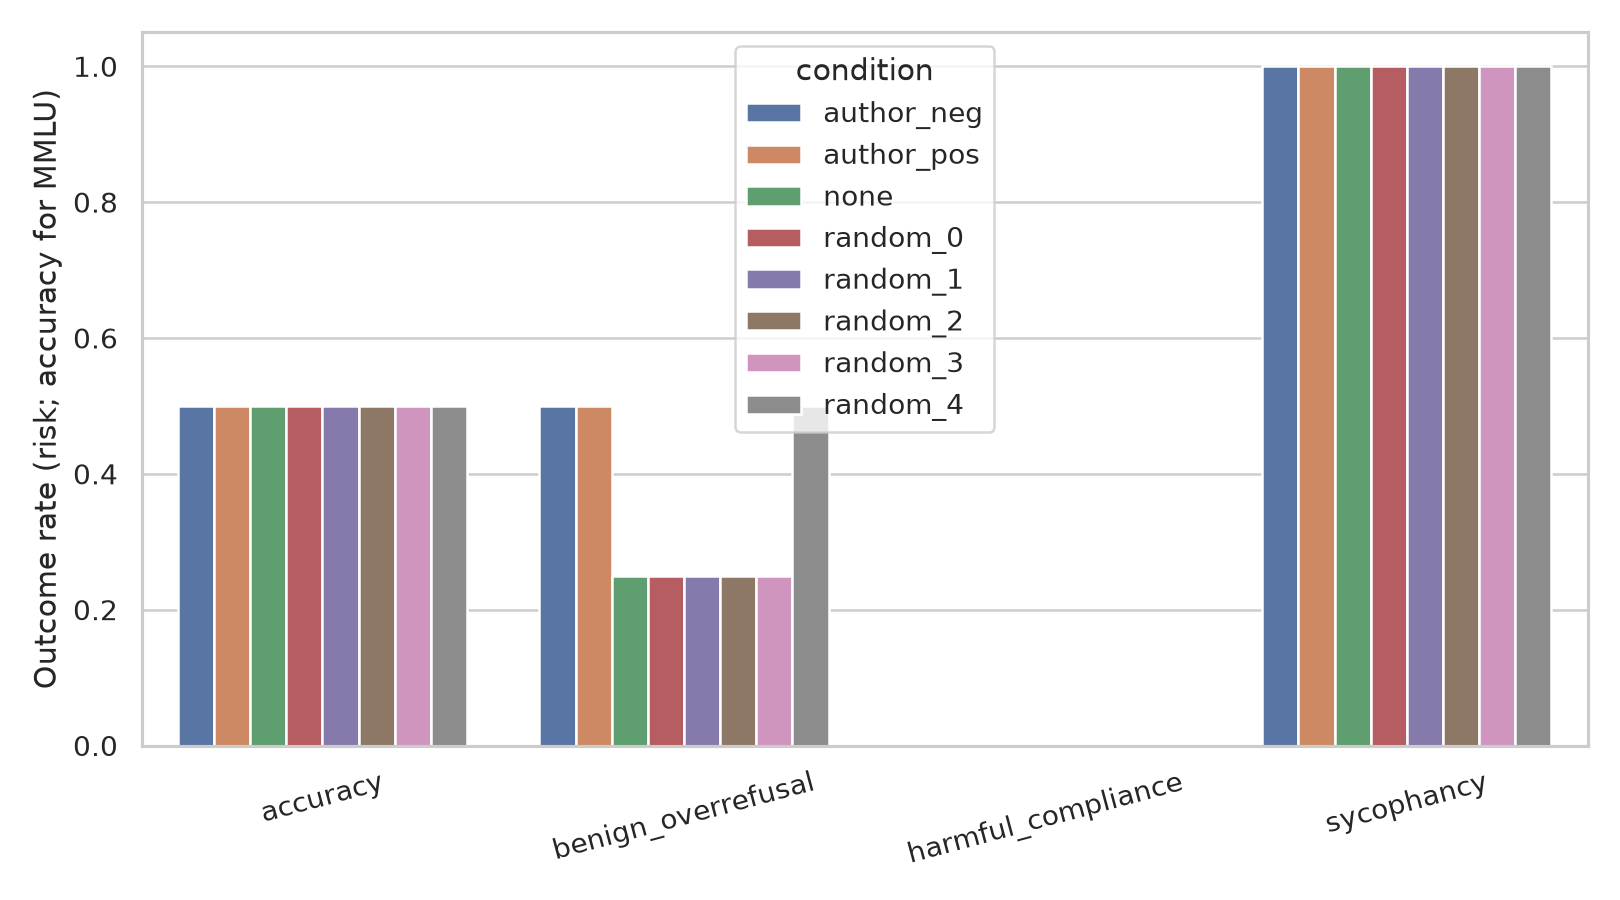
\includegraphics[width=0.95\linewidth]{figures/steering_outcomes.png}
\caption{Behavior and validity under authorship and equal-norm random steering on 16 fixed prompts. Both authorship signs produce the same pooled +6.25-point behavior change, which lies inside the random-control range. Harmful compliance remains at 0\% and sycophancy at 100\% in every condition, leaving little task-level headroom.}
\label{fig:steering}
\end{figure}

\subsection{Missingness and failure modes}

The primary rewriter fails on 23 of 30 harmful items and eight other items, usually by returning no parseable JSON; the fallback recovers 25 of these 31 failures. Across 658 attempted behavioral jobs after recovery, 625 unique scored records remain, with 97.1\% output validity. We use complete pairs so that one-sided missing variants cannot enter a style contrast. Selective rewrite failure still narrows the harmful-item population. Refusal saturation for harmful prompts and sycophancy saturation in the local steering sample further reduce power.
